% Options for packages loaded elsewhere
\PassOptionsToPackage{unicode}{hyperref}
\PassOptionsToPackage{hyphens}{url}
\PassOptionsToPackage{dvipsnames,svgnames,x11names}{xcolor}
%
\documentclass[
  12pt,
]{article}

\usepackage{amsmath,amssymb}
\usepackage{lmodern}
\usepackage{iftex}
\ifPDFTeX
  \usepackage[T1]{fontenc}
  \usepackage[utf8]{inputenc}
  \usepackage{textcomp} % provide euro and other symbols
\else % if luatex or xetex
  \usepackage{unicode-math}
  \defaultfontfeatures{Scale=MatchLowercase}
  \defaultfontfeatures[\rmfamily]{Ligatures=TeX,Scale=1}
\fi
% Use upquote if available, for straight quotes in verbatim environments
\IfFileExists{upquote.sty}{\usepackage{upquote}}{}
\IfFileExists{microtype.sty}{% use microtype if available
  \usepackage[]{microtype}
  \UseMicrotypeSet[protrusion]{basicmath} % disable protrusion for tt fonts
}{}
\makeatletter
\@ifundefined{KOMAClassName}{% if non-KOMA class
  \IfFileExists{parskip.sty}{%
    \usepackage{parskip}
  }{% else
    \setlength{\parindent}{0pt}
    \setlength{\parskip}{6pt plus 2pt minus 1pt}}
}{% if KOMA class
  \KOMAoptions{parskip=half}}
\makeatother
\usepackage{xcolor}
\usepackage[top=1in,left=1in,bottom=1in,right=1in]{geometry}
\setlength{\emergencystretch}{3em} % prevent overfull lines
\setcounter{secnumdepth}{-\maxdimen} % remove section numbering
% Make \paragraph and \subparagraph free-standing
\ifx\paragraph\undefined\else
  \let\oldparagraph\paragraph
  \renewcommand{\paragraph}[1]{\oldparagraph{#1}\mbox{}}
\fi
\ifx\subparagraph\undefined\else
  \let\oldsubparagraph\subparagraph
  \renewcommand{\subparagraph}[1]{\oldsubparagraph{#1}\mbox{}}
\fi


\providecommand{\tightlist}{%
  \setlength{\itemsep}{0pt}\setlength{\parskip}{0pt}}\usepackage{longtable,booktabs,array}
\usepackage{calc} % for calculating minipage widths
% Correct order of tables after \paragraph or \subparagraph
\usepackage{etoolbox}
\makeatletter
\patchcmd\longtable{\par}{\if@noskipsec\mbox{}\fi\par}{}{}
\makeatother
% Allow footnotes in longtable head/foot
\IfFileExists{footnotehyper.sty}{\usepackage{footnotehyper}}{\usepackage{footnote}}
\makesavenoteenv{longtable}
\usepackage{graphicx}
\makeatletter
\def\maxwidth{\ifdim\Gin@nat@width>\linewidth\linewidth\else\Gin@nat@width\fi}
\def\maxheight{\ifdim\Gin@nat@height>\textheight\textheight\else\Gin@nat@height\fi}
\makeatother
% Scale images if necessary, so that they will not overflow the page
% margins by default, and it is still possible to overwrite the defaults
% using explicit options in \includegraphics[width, height, ...]{}
\setkeys{Gin}{width=\maxwidth,height=\maxheight,keepaspectratio}
% Set default figure placement to htbp
\makeatletter
\def\fps@figure{htbp}
\makeatother
\newlength{\cslhangindent}
\setlength{\cslhangindent}{1.5em}
\newlength{\csllabelwidth}
\setlength{\csllabelwidth}{3em}
\newlength{\cslentryspacingunit} % times entry-spacing
\setlength{\cslentryspacingunit}{\parskip}
\newenvironment{CSLReferences}[2] % #1 hanging-ident, #2 entry spacing
 {% don't indent paragraphs
  \setlength{\parindent}{0pt}
  % turn on hanging indent if param 1 is 1
  \ifodd #1
  \let\oldpar\par
  \def\par{\hangindent=\cslhangindent\oldpar}
  \fi
  % set entry spacing
  \setlength{\parskip}{#2\cslentryspacingunit}
 }%
 {}
\usepackage{calc}
\newcommand{\CSLBlock}[1]{#1\hfill\break}
\newcommand{\CSLLeftMargin}[1]{\parbox[t]{\csllabelwidth}{#1}}
\newcommand{\CSLRightInline}[1]{\parbox[t]{\linewidth - \csllabelwidth}{#1}\break}
\newcommand{\CSLIndent}[1]{\hspace{\cslhangindent}#1}

\usepackage{booktabs}
\usepackage{longtable}
\usepackage{array}
\usepackage{multirow}
\usepackage{wrapfig}
\usepackage{float}
\usepackage{colortbl}
\usepackage{pdflscape}
\usepackage{tabu}
\usepackage{threeparttable}
\usepackage{threeparttablex}
\usepackage[normalem]{ulem}
\usepackage{makecell}
\usepackage{xcolor}
\usepackage[noblocks]{authblk}
\renewcommand*{\Authsep}{, }
\renewcommand*{\Authand}{, }
\renewcommand*{\Authands}{, }
\renewcommand\Affilfont{\normalsize}
\usepackage{lineno}\linenumbers
\usepackage{sectsty}\sectionfont{\centering}
\usepackage{sectsty}\subsectionfont{\centering}
\usepackage{fontspec}
\usepackage{titlesec}
\makeatletter
\makeatother
\makeatletter
\makeatother
\makeatletter
\@ifpackageloaded{caption}{}{\usepackage{caption}}
\AtBeginDocument{%
\ifdefined\contentsname
  \renewcommand*\contentsname{Table of contents}
\else
  \newcommand\contentsname{Table of contents}
\fi
\ifdefined\listfigurename
  \renewcommand*\listfigurename{List of Figures}
\else
  \newcommand\listfigurename{List of Figures}
\fi
\ifdefined\listtablename
  \renewcommand*\listtablename{List of Tables}
\else
  \newcommand\listtablename{List of Tables}
\fi
\ifdefined\figurename
  \renewcommand*\figurename{Figure}
\else
  \newcommand\figurename{Figure}
\fi
\ifdefined\tablename
  \renewcommand*\tablename{Table}
\else
  \newcommand\tablename{Table}
\fi
}
\@ifpackageloaded{float}{}{\usepackage{float}}
\floatstyle{ruled}
\@ifundefined{c@chapter}{\newfloat{codelisting}{h}{lop}}{\newfloat{codelisting}{h}{lop}[chapter]}
\floatname{codelisting}{Listing}
\newcommand*\listoflistings{\listof{codelisting}{List of Listings}}
\makeatother
\makeatletter
\@ifpackageloaded{caption}{}{\usepackage{caption}}
\@ifpackageloaded{subcaption}{}{\usepackage{subcaption}}
\makeatother
\makeatletter
\@ifpackageloaded{tcolorbox}{}{\usepackage[many]{tcolorbox}}
\makeatother
\makeatletter
\@ifundefined{shadecolor}{\definecolor{shadecolor}{rgb}{.97, .97, .97}}
\makeatother
\makeatletter
\makeatother
\ifLuaTeX
  \usepackage{selnolig}  % disable illegal ligatures
\fi
\IfFileExists{bookmark.sty}{\usepackage{bookmark}}{\usepackage{hyperref}}
\IfFileExists{xurl.sty}{\usepackage{xurl}}{} % add URL line breaks if available
\urlstyle{same} % disable monospaced font for URLs
\hypersetup{
  pdftitle={Context-dependent consequences of including lagged effects in demographic models},
  pdfkeywords={integral projection models, environmental
stochasticity, lagged effects},
  colorlinks=true,
  linkcolor={blue},
  filecolor={Maroon},
  citecolor={Blue},
  urlcolor={Blue},
  pdfcreator={LaTeX via pandoc}}

\title{Context-dependent consequences of including lagged effects in
demographic models}


\author[1]{Eric R. Scott}
\author{María Uriarte}
\author[1,3,5]{Emilio M. Bruna}

\affil[1]{Department of Wildlife Ecology and Conservation, University of
Florida, Gainesville, Florida 32611-0430 USA}
\affil[2]{Department of Ecology, Evolution and Environmental Biology,
Columbia University 1200 Amsterdam Avenue, New York, New York 10027 USA}
\affil[3]{Center for Latin American Studies, University of Florida,
Gainesville, Florida 32611-5530 USA}
\affil[4]{Biological Dynamics of Forest Fragments Project, INPA-PDBFF,
CP 478, Manaus, Amazonas 69011-970 Brazil}


\date{(draft: 21 July 2023)}
\begin{document}
\maketitle
\ifdefined\Shaded\renewenvironment{Shaded}{\begin{tcolorbox}[enhanced, borderline west={3pt}{0pt}{shadecolor}, breakable, sharp corners, boxrule=0pt, interior hidden, frame hidden]}{\end{tcolorbox}}\fi

\pagebreak

\hypertarget{abstract}{%
\section{Abstract}\label{abstract}}

Text of 150 words max summarizing this amazing paper.

\pagebreak

\hypertarget{introduction}{%
\subsection{Introduction}\label{introduction}}

\hypertarget{paragraph-1}{%
\subsubsection{\texorpdfstring{\textbf{Paragraph
1}}{Paragraph 1}}\label{paragraph-1}}

\begin{enumerate}
\def\labelenumi{\arabic{enumi}.}
\tightlist
\item
  Structured demographic models, such as Integral Projection Models
  (IPMs) and matrix models, have emerged as invaluable tools in ecology,
  evolution, and conservation biology.
\end{enumerate}

They provide insights into \_\_\_\_, the evolution of life-history
strategies, and life-history stages and ecological processes at which
conservation intervention is likely to have the greatest impact on
population growth rate.

Their flexibility hasmade them increasingly applicable to species with
differtent life histories.

however, there are still a number of challenges to address, namely
\_\_\_\_ , \_\_\_\_, and \_\_\_\_.

\hypertarget{paragraph-2}{%
\subsubsection{\texorpdfstring{\textbf{Paragraph
2}}{Paragraph 2}}\label{paragraph-2}}

\begin{enumerate}
\def\labelenumi{\arabic{enumi}.}
\tightlist
\item
  It has long been recognized that there is the potential for lagged
  effects.
\item
  Including lagged effects in models has been a major technical
  challenge, but there are now multiple approaches for doing so.
\item
  The studies assessing the potential for lagged effects on vital rates
  find that they indeed appear to be prevalent (Evers et al. 2021; Scott
  et al. 2022).
\end{enumerate}

\hypertarget{paragraph-3}{%
\subsubsection{\texorpdfstring{\textbf{Paragraph
3}}{Paragraph 3}}\label{paragraph-3}}

\begin{enumerate}
\def\labelenumi{\arabic{enumi}.}
\tightlist
\item
  Lagged effects could be different in different habitat types.
\item
  This could be a big reason for differences between habitats.
\end{enumerate}

\hypertarget{paragraph-4}{%
\subsubsection{\texorpdfstring{\textbf{Paragraph
4}}{Paragraph 4}}\label{paragraph-4}}

\begin{enumerate}
\def\labelenumi{\arabic{enumi}.}
\tightlist
\item
  Here we\ldots{}
\item
  We conducted these analyses with both deterministic and stochastic
  IPMs.
\end{enumerate}

\hypertarget{methods}{%
\subsection{Methods}\label{methods}}

\hypertarget{demographic-methods-and-data}{%
\subsubsection{\texorpdfstring{\emph{Demographic methods and
data}}{Demographic methods and data}}\label{demographic-methods-and-data}}

Overview of the heliconia project and data

\hypertarget{construction-of-integral-projection-models}{%
\subsubsection{\texorpdfstring{\emph{Construction of Integral Projection
Models}}{Construction of Integral Projection Models}}\label{construction-of-integral-projection-models}}

In preliminary investigation we found that the survival and growth of
plants was better explained by treating seedlings and mature plants
separately. Seedlings are physiologically different from small plants
because they necessarily lack the underground reserves (of carbohydrates
and meristems) that a small, mature plant may have. Therefore, we used
general IPMs to model population dynamics with seedlings treated as a
separate discreet class not structured by size. General IPMs allow for
combinations of continuous and discrete states and transitions between
them (Ellner et al. 2016).

We built three classes of IPMs for comparison which each required
different functional forms of their underlying vital rates models. The
simplest IPM was a general, density-independent, deterministic IPM with
four sub-kernels: growth and survival (\(P\), Equation~\ref{eq-P}),
fecundity (\(F\), i.e.~production of new seedlings,
Equation~\ref{eq-F}), probability of staying a seedling (always 0), and
recruitment (\(R\), i.e.~seedling survival and establishment,
Equation~\ref{eq-R}) (Equation~\ref{eq-mature}, Equation~\ref{eq-sdlg},
Figure~\ref{fig-lifecycle}). The probability of staying a seedling, was
always equal to zero, since our definition of seedlings was first year
plants only.

\begin{equation}\protect\hypertarget{eq-mature}{}{
n(z^{\prime},t+1) = R(z^\prime)n_s(t) + \int_L^U P(z^\prime,z) n(z,t)\;dz
}\label{eq-mature}\end{equation}

\begin{equation}\protect\hypertarget{eq-sdlg}{}{
n_s(t+1) = \int_L^U F(z) n(z,t) \; dz
}\label{eq-sdlg}\end{equation}

\begin{equation}\protect\hypertarget{eq-R}{}{
R(z^\prime) = s_sG_s(z^\prime)
}\label{eq-R}\end{equation}

\begin{equation}\protect\hypertarget{eq-P}{}{
P(z^\prime, z) = s(z)G(z^\prime, z)
}\label{eq-P}\end{equation}

\begin{equation}\protect\hypertarget{eq-F}{}{
F(z) = p_f(z)f(z)g
}\label{eq-F}\end{equation}

The number and size of mature plants in the next census is determined by
seedlings entering the mature plant population (i.e.~recruitment ) and
survival and growth (or regression) of mature plants
(Equation~\ref{eq-mature}). Seedlings survive (\(s_s\)) and grow into
mature plants of a particular size (\(G_s(z^\prime)\))
(Equation~\ref{eq-R}). Mature plants survive as a function of size
(\(s(z)\)), and grow (or regress) to a new size as a function of their
previous size (\(G(z^\prime, z)\)) (Equation~\ref{eq-P}). Mature plants
flower with a probability that is a function of size (\(p_f(z)\)) and
produce a number of seeds as a function of size (\(f(z)\)), which
germinate and establish as seedlings with probability \(g\)
(Equation~\ref{eq-F}).

Vital rate models for growth (\(G_s(z^\prime)\) and \(G(z^\prime, z)\))
, survival (\(s_s\) and \(s(z)\)), and flowering (\(p_f(z)\)) were fit
using the long term demographic dataset. For established plants, these
three vital rates were modeled as a smooth function of size in the
previous census using generalized additive models (GAMs) fit with the
\texttt{mgcv} package(Wood 2011) in R version 4.3.0 (2023-04-21) (R Core
Team 2020) . For consistency, seedling survival and growth were also
modeled using GAMs, but without size in the previous census as a
predictor (i.e.~intercept only models). For growth models
(\(G_s(z^\prime)\) and \(G(z^\prime, z)\)) a scaled t family
distribution provided a better fit to the data than a gaussian fit as
the residuals were leptokurtic with a simple gaussian model.

To estimate reproduction we drew on additional data sources to estimate
the number of fruits per flowering plant as a function of plant size and
the number of seeds per fruit (together \(f(z)\)). Germination and
establishment rates in continuous forest and forest fragments were
estimated using data from \ldots.

To build the general, density-independent, stochastic, kernel-resampled
IPMs, we included environmental stochasticity in all vital rate models
built using the long term demographic datset by adding a random effect
of year (Figure~\ref{fig-lifecycle}). The random effect of year was
included using a factor--smooth interaction which allowed the
relationship between plant size and vital rates to vary in functional
form among transition years. The kernel-resampling approach is to
generate kernels corresponding to each transition year in the
demographic dataset using the random smooths for year, and to iterate
the IPM by drawing from these randomly. This is equivalent to the matrix
selection approach for matrix population models described by Caswell
(2001).

For the third method, we modeled the impacts of drought on vital rates
explicitly and created general, density-independent, stochastic,
parameter-resampled IPMs (\emph{sensu} Metcalf et al. (2015)). We
calculated the standardized precipitation evapotranspiraton index (SPEI)
for our site using a published gridded dataset based on ground
measurements (Xavier et al. 2016) as described in Scott et al. (2022).
For all vital rate models fit using the long term demographic dataset,
we modeled delayed effects of SPEI using distributed lag non-linear
models with a maximum lag of 36 months (Scott et al. 2022)
(Figure~\ref{fig-lifecycle}). To iterate these parameter-resampled IPMs,
a random sequence of SPEI values was created by sampling years of the
observed monthly SPEI data. Then, 36 month lags are calculated for each
year starting in February (the month of the demographic census). These
values are then used to predict fitted values from the vital rates
models, generating different kernels at each iteration of the IPM. With
this method, the kernels of successive iterations are not entirely
independent because the SPEI values used in calculating vital rates
include values used in the previous two iterations, but they are
ergodic.

All IPMs were constructed and iterated using the \texttt{ipmr} package
in R (Levin et al. 2021). The IPMs used 100 meshpoints and the midpoint
rule for calculating kernels . For each type of IPM we iterated the
model for 1000 time steps, discarding the first 100 time steps to omit
transient effects. Stochastic growth rates (\(\lambda_s\)) were
calculated as the average \(ln(\lambda)\) from each time step (Caswell
2001) and back-transformed to be on the same scale as deterministic
lambdas for comparison. We used the distribution of established plant
sizes and proportion of seedlings from the full dataset as a starting
population vector. While other starting population vectors were
possible, the choice is of little importance as it will only impact
transient dynamics, which we aren't interested in for this study.

To estimate uncertainty around the per-capita growth rates (lambdas), we
created 500 bootstraps of the demographic dataset by sampling individual
plants with replacement within each habitat. For each bootstrap, we then
re-fit vital rates models (all except germination and establishment
rate, fruits per flowering plant, and seeds per fruit, which were
estimated using different datasets), constructed IPMs, and calculated a
value for lambda as described above. We then used these bootstraped
estimates of lambda to calculate bias corrected 95\% confidence
intervals (Ellner et al. 2016).

This workflow was managed using the \texttt{targets} R package (Landau
2021) which also allowed us to track computational time spent on each
IPM for comparison.

\hypertarget{statistical-analyses}{%
\subsubsection{\texorpdfstring{\emph{Statistical
analyses}}{Statistical analyses}}\label{statistical-analyses}}

All about the stats.

\hypertarget{results}{%
\subsection{Results}\label{results}}

For all vital rates estimated using the long term demographic dataset,
the DLNM model fit the best (dAIC = 0) followed by the model with a
random effect of year, followed by the deterministic model
(Table~\ref{tbl-aic}).\\

Population growth rates were consistently higher in continuous forest
compared to forest fragments across IPM types (Table~\ref{tbl-lambdas}).

The time to iterate the DLNM models is much higher than than
deterministic and kernel-resampled.

The greater use of computational resources is likely a result of
\texttt{predict()} being much slower for GAMs with 2D smooths because
the number of knots is much higher compared to the GAMs used for the
vital rates models in the determinsitic and kernel-resampled IPMs.

Figure~\ref{fig-pop-states} has some interesting things in it:

\begin{itemize}
\item
  for the deterministic IPM (and the kernel-resampled IPM?) there are
  slightly more of the smallest plants and the largest plants in CF
  compared to FF (i.e.~more medium sized plants in FF).
\item
  For the kernel-resampled IPM (random effect of year), the fluctuations
  are extremely similar between CF and FF
\item
  For the parameter-resampled IPM (DLNM) the size structure of the
  population is a LOT more variable in FF. This makes sense as we know
  lagged effects are more important in fragments.
\item
  Also, the fluctuations in size structure in CF do not match the
  fluctuations in FF as well (can see this by the increased spread of
  points in Figure~\ref{fig-pop-states} (B)
\item
  Also, in the parameter-resampled IPM (and only in this one), we see a
  shift toward smaller plants in FF compared to CF
\end{itemize}

\hypertarget{discussion}{%
\subsection{Discussion}\label{discussion}}

\begin{itemize}
\tightlist
\item
  Our finding that the choice of IPM didn't change the relative ranking
  of CF and FF is consistent with Kaye and Pyke (2003) finding that
  method effected stochastic lambda, but relative ranking of populations
  was consistent.
\end{itemize}

\hypertarget{acknowledgments}{%
\subsection{Acknowledgments}\label{acknowledgments}}

We thank \textbf{,} \_, \_\_\_ and \_\_\_ anonymous reviewers for
helpful discussions and comments on the manuscript. We thank Sam Levin
for his help with the \texttt{ipmr} package. Financial support was
provided by the U.S. National Science Foundation (awards \_\_\_\_, and
\_\_\_\_). This article is publication no. -- -- in the BDFFP Technical
series. The authors declare no conflicts of interest.

\hypertarget{credit-statement}{%
\subsection{CRediT Statement}\label{credit-statement}}

ERS contributed to the conceptualization, methodology, formal analysis,
and led the writing of the original draft. EMB contributed to the
conceptualization, methodology, and writing and also acquired funding.

\hypertarget{data-availability-statement}{%
\subsection{Data Availability
Statement}\label{data-availability-statement}}

Data and R code used in this study are archived with Zenodo at .

\hypertarget{literature-cited}{%
\subsection{Literature Cited}\label{literature-cited}}

\hypertarget{refs}{}
\begin{CSLReferences}{0}{0}
\leavevmode\vadjust pre{\hypertarget{ref-caswell2001}{}}%
Caswell, H. 2001. Matrix population models: Construction, analysis, and
interpretation. Sinauer Associates, Sunderland.

\leavevmode\vadjust pre{\hypertarget{ref-ellnerDatadrivenModellingStructured2016}{}}%
Ellner, S. P., D. Z. Childs, and M. Rees. 2016. Data-driven modelling of
structured populations: A practical guide to the integral projection
model. {Springer Science+Business Media}, {New York, NY}.

\leavevmode\vadjust pre{\hypertarget{ref-eversLaggedDormantSeason2021}{}}%
Evers, S. M., T. M. Knight, D. W. Inouye, T. E. X. Miller, R.
Salguero-Gómez, A. M. Iler, and A. Compagnoni. 2021.
\href{https://doi.org/10.1111/gcb.15519}{Lagged and dormant season
climate better predict plant vital rates than climate during the growing
season}. Global Change Biology 27:1927--1941.

\leavevmode\vadjust pre{\hypertarget{ref-kayeEffectStochasticTechnique2003}{}}%
Kaye, T. N., and D. A. Pyke. 2003.
\href{https://doi.org/10.1890/0012-9658(2003)084\%5B1464:TEOSTO\%5D2.0.CO;2}{The
effect of stochastic technique on estimates of population viability from
transition matrix models}. Ecology 84:1464--1476.

\leavevmode\vadjust pre{\hypertarget{ref-targets}{}}%
Landau, W. M. 2021. \href{https://doi.org/10.21105/joss.02959}{The
targets r package: A dynamic make-like function-oriented pipeline
toolkit for reproducibility and high-performance computing} 6:2959.

\leavevmode\vadjust pre{\hypertarget{ref-levinIpmrFlexibleImplementation2021}{}}%
Levin, S. C., D. Z. Childs, A. Compagnoni, S. Evers, T. M. Knight, and
R. Salguero-Gómez. 2021.
\href{https://doi.org/10.1111/2041-210X.13683}{Ipmr: {Flexible}
implementation of {Integral Projection Models} in {R}}. Methods in
Ecology and Evolution 12:1826--1834.

\leavevmode\vadjust pre{\hypertarget{ref-metcalfStatisticalModellingAnnual2015}{}}%
Metcalf, C. J. E., S. P. Ellner, D. Z. Childs, R. Salguero-Gómez, C.
Merow, S. M. McMahon, E. Jongejans, et al. 2015.
\href{https://doi.org/10.1111/2041-210X.12405}{Statistical modelling of
annual variation for inference on stochastic population dynamics using
{Integral Projection Models}}. Methods in Ecology and Evolution
6:1007--1017.

\leavevmode\vadjust pre{\hypertarget{ref-rcoreteam2020}{}}%
R Core Team. 2020. \emph{R: {A} language and environment for statistical
computing}. {Vienna, Austria}.

\leavevmode\vadjust pre{\hypertarget{ref-scottDelayedEffectsClimate2022}{}}%
Scott, E. R., M. Uriarte, and E. M. Bruna. 2022.
\href{https://doi.org/10.1111/gcb.15900}{Delayed effects of climate on
vital rates lead to demographic divergence in Amazonian forest
fragments}. Global Change Biology 28:463--479.

\leavevmode\vadjust pre{\hypertarget{ref-mgcv}{}}%
Wood, S. N. 2011. Fast stable restricted maximum likelihood and marginal
likelihood estimation of semiparametric generalized linear models
73:3--36.

\leavevmode\vadjust pre{\hypertarget{ref-xavierDailyGriddedMeteorological2016}{}}%
Xavier, A. C., C. W. King, and B. R. Scanlon. 2016.
\href{https://doi.org/10.1002/joc.4518}{Daily gridded meteorological
variables in {Brazil} (1980\textendash 2013)}. International Journal of
Climatology 36:2644--2659.

\end{CSLReferences}

\pagebreak

\hypertarget{tbl-aic}{}
\begin{longtable}[]{@{}
  >{\raggedright\arraybackslash}p{(\columnwidth - 8\tabcolsep) * \real{0.1389}}
  >{\raggedright\arraybackslash}p{(\columnwidth - 8\tabcolsep) * \real{0.2778}}
  >{\raggedright\arraybackslash}p{(\columnwidth - 8\tabcolsep) * \real{0.3333}}
  >{\raggedleft\arraybackslash}p{(\columnwidth - 8\tabcolsep) * \real{0.1111}}
  >{\raggedleft\arraybackslash}p{(\columnwidth - 8\tabcolsep) * \real{0.1111}}@{}}
\caption{\label{tbl-aic}Comparison of vital rate models used to build
IPM. The `Effect of Environment' column describes how environmental
effects were included in models. Those with `none' were used to build
deterministic IPMs; those with a random effect of year were used to
build stochastic, kernel-resampled IPMs; and those with a distributed
lag non-linear model (DLNM) were used to build stochastic,
parameter-resampled IPMs. `edf' is the estimated degrees of freedom of
the penalized GAM. ΔAIC is calculated within each habitat and vital rate
combination. ΔAIC within 2 indicates models are
equivalent.}\tabularnewline
\toprule()
\begin{minipage}[b]{\linewidth}\raggedright
Habitat
\end{minipage} & \begin{minipage}[b]{\linewidth}\raggedright
Vital Rate
\end{minipage} & \begin{minipage}[b]{\linewidth}\raggedright
Effect of Environment
\end{minipage} & \begin{minipage}[b]{\linewidth}\raggedleft
edf
\end{minipage} & \begin{minipage}[b]{\linewidth}\raggedleft
ΔAIC
\end{minipage} \\
\midrule()
\endfirsthead
\toprule()
\begin{minipage}[b]{\linewidth}\raggedright
Habitat
\end{minipage} & \begin{minipage}[b]{\linewidth}\raggedright
Vital Rate
\end{minipage} & \begin{minipage}[b]{\linewidth}\raggedright
Effect of Environment
\end{minipage} & \begin{minipage}[b]{\linewidth}\raggedleft
edf
\end{minipage} & \begin{minipage}[b]{\linewidth}\raggedleft
ΔAIC
\end{minipage} \\
\midrule()
\endhead
CF & Survival & Random effect of year & 43.26 & 0 \\
CF & Survival & DLNM & 19.72 & 78.92 \\
CF & Survival & None & 4.976 & 260 \\
CF & Growth & Random effect of year & 78.43 & 0 \\
CF & Growth & DLNM & 23.87 & 158.5 \\
CF & Growth & None & 7.81 & 1896 \\
CF & Flowering & DLNM & 19.59 & 0 \\
CF & Flowering & Random effect of year & 17.19 & 1.627 \\
CF & Flowering & None & 7.468 & 381.9 \\
CF & Seedling survival & None & 1 & 0 \\
CF & Seedling survival & Random effect of year & 1.817 & 1.386 \\
CF & Seedling survival & DLNM & 4.008 & 1.528 \\
CF & Seedling growth & Random effect of year & 9.475 & 0 \\
CF & Seedling growth & DLNM & 8.952 & 2.902 \\
CF & Seedling growth & None & 1 & 172.3 \\
FF & Survival & DLNM & 14.95 & 0 \\
FF & Survival & Random effect of year & 19.21 & 35.68 \\
FF & Survival & None & 4.333 & 51.25 \\
FF & Growth & DLNM & 25.18 & 0 \\
FF & Growth & Random effect of year & 37.84 & 200 \\
FF & Growth & None & 5.599 & 382.8 \\
FF & Flowering & DLNM & 20.61 & 0 \\
FF & Flowering & Random effect of year & 13.81 & 27.4 \\
FF & Flowering & None & 5.007 & 101.7 \\
FF & Seedling survival & DLNM & 5.574 & 0 \\
FF & Seedling survival & Random effect of year & 5.088 & 5.721 \\
FF & Seedling survival & None & 1 & 6.491 \\
FF & Seedling growth & Random effect of year & 6.25 & 0 \\
FF & Seedling growth & DLNM & 8.182 & 2.29 \\
FF & Seedling growth & None & 1 & 5.745 \\
\bottomrule()
\end{longtable}

\newpage

\hypertarget{tbl-time}{}
\begin{table}
\caption{\label{tbl-time}Figure caption to be written }\tabularnewline

\centering
\begin{tabular}[t]{lc}
\toprule
IPM Type & mean time (min.)\\
\midrule
Deterministic & 0.02\\
Stochastic, kernel-resampled & 0.07\\
Stochastic, parameter-resampled & 87.12\\
\bottomrule
\end{tabular}
\end{table}

\newpage

\hypertarget{tbl-lambdas}{}
\begin{longtable}[]{@{}
  >{\raggedright\arraybackslash}p{(\columnwidth - 4\tabcolsep) * \real{0.4306}}
  >{\raggedright\arraybackslash}p{(\columnwidth - 4\tabcolsep) * \real{0.1389}}
  >{\raggedleft\arraybackslash}p{(\columnwidth - 4\tabcolsep) * \real{0.3611}}@{}}
\caption{\label{tbl-lambdas}Population growth rates for continuous
forest (CF) and forest fragments (FF) under different kinds of IPMs with
bootstrapped, bias-corrected, 95\% confidence intervals.}\tabularnewline
\toprule()
\begin{minipage}[b]{\linewidth}\raggedright
IPM
\end{minipage} & \begin{minipage}[b]{\linewidth}\raggedright
Habitat
\end{minipage} & \begin{minipage}[b]{\linewidth}\raggedleft
\(\lambda\)
\end{minipage} \\
\midrule()
\endfirsthead
\toprule()
\begin{minipage}[b]{\linewidth}\raggedright
IPM
\end{minipage} & \begin{minipage}[b]{\linewidth}\raggedright
Habitat
\end{minipage} & \begin{minipage}[b]{\linewidth}\raggedleft
\(\lambda\)
\end{minipage} \\
\midrule()
\endhead
Deterministic & FF & 0.9778 (0.9736, 0.9823) \\
Deterministic & CF & 0.9897 (0.9877, 0.9920) \\
Stochastic, kernel-resampled & FF & 0.9787 (0.9735, 0.9835) \\
Stochastic, kernel-resampled & CF & 0.9913 (0.9892, 0.9939) \\
dlnm & FF & 0.9595 (0.9459, 0.9689) \\
dlnm & CF & 0.9795 (0.9752, 0.9867) \\
\bottomrule()
\end{longtable}

\newpage

\begin{figure}

{\centering 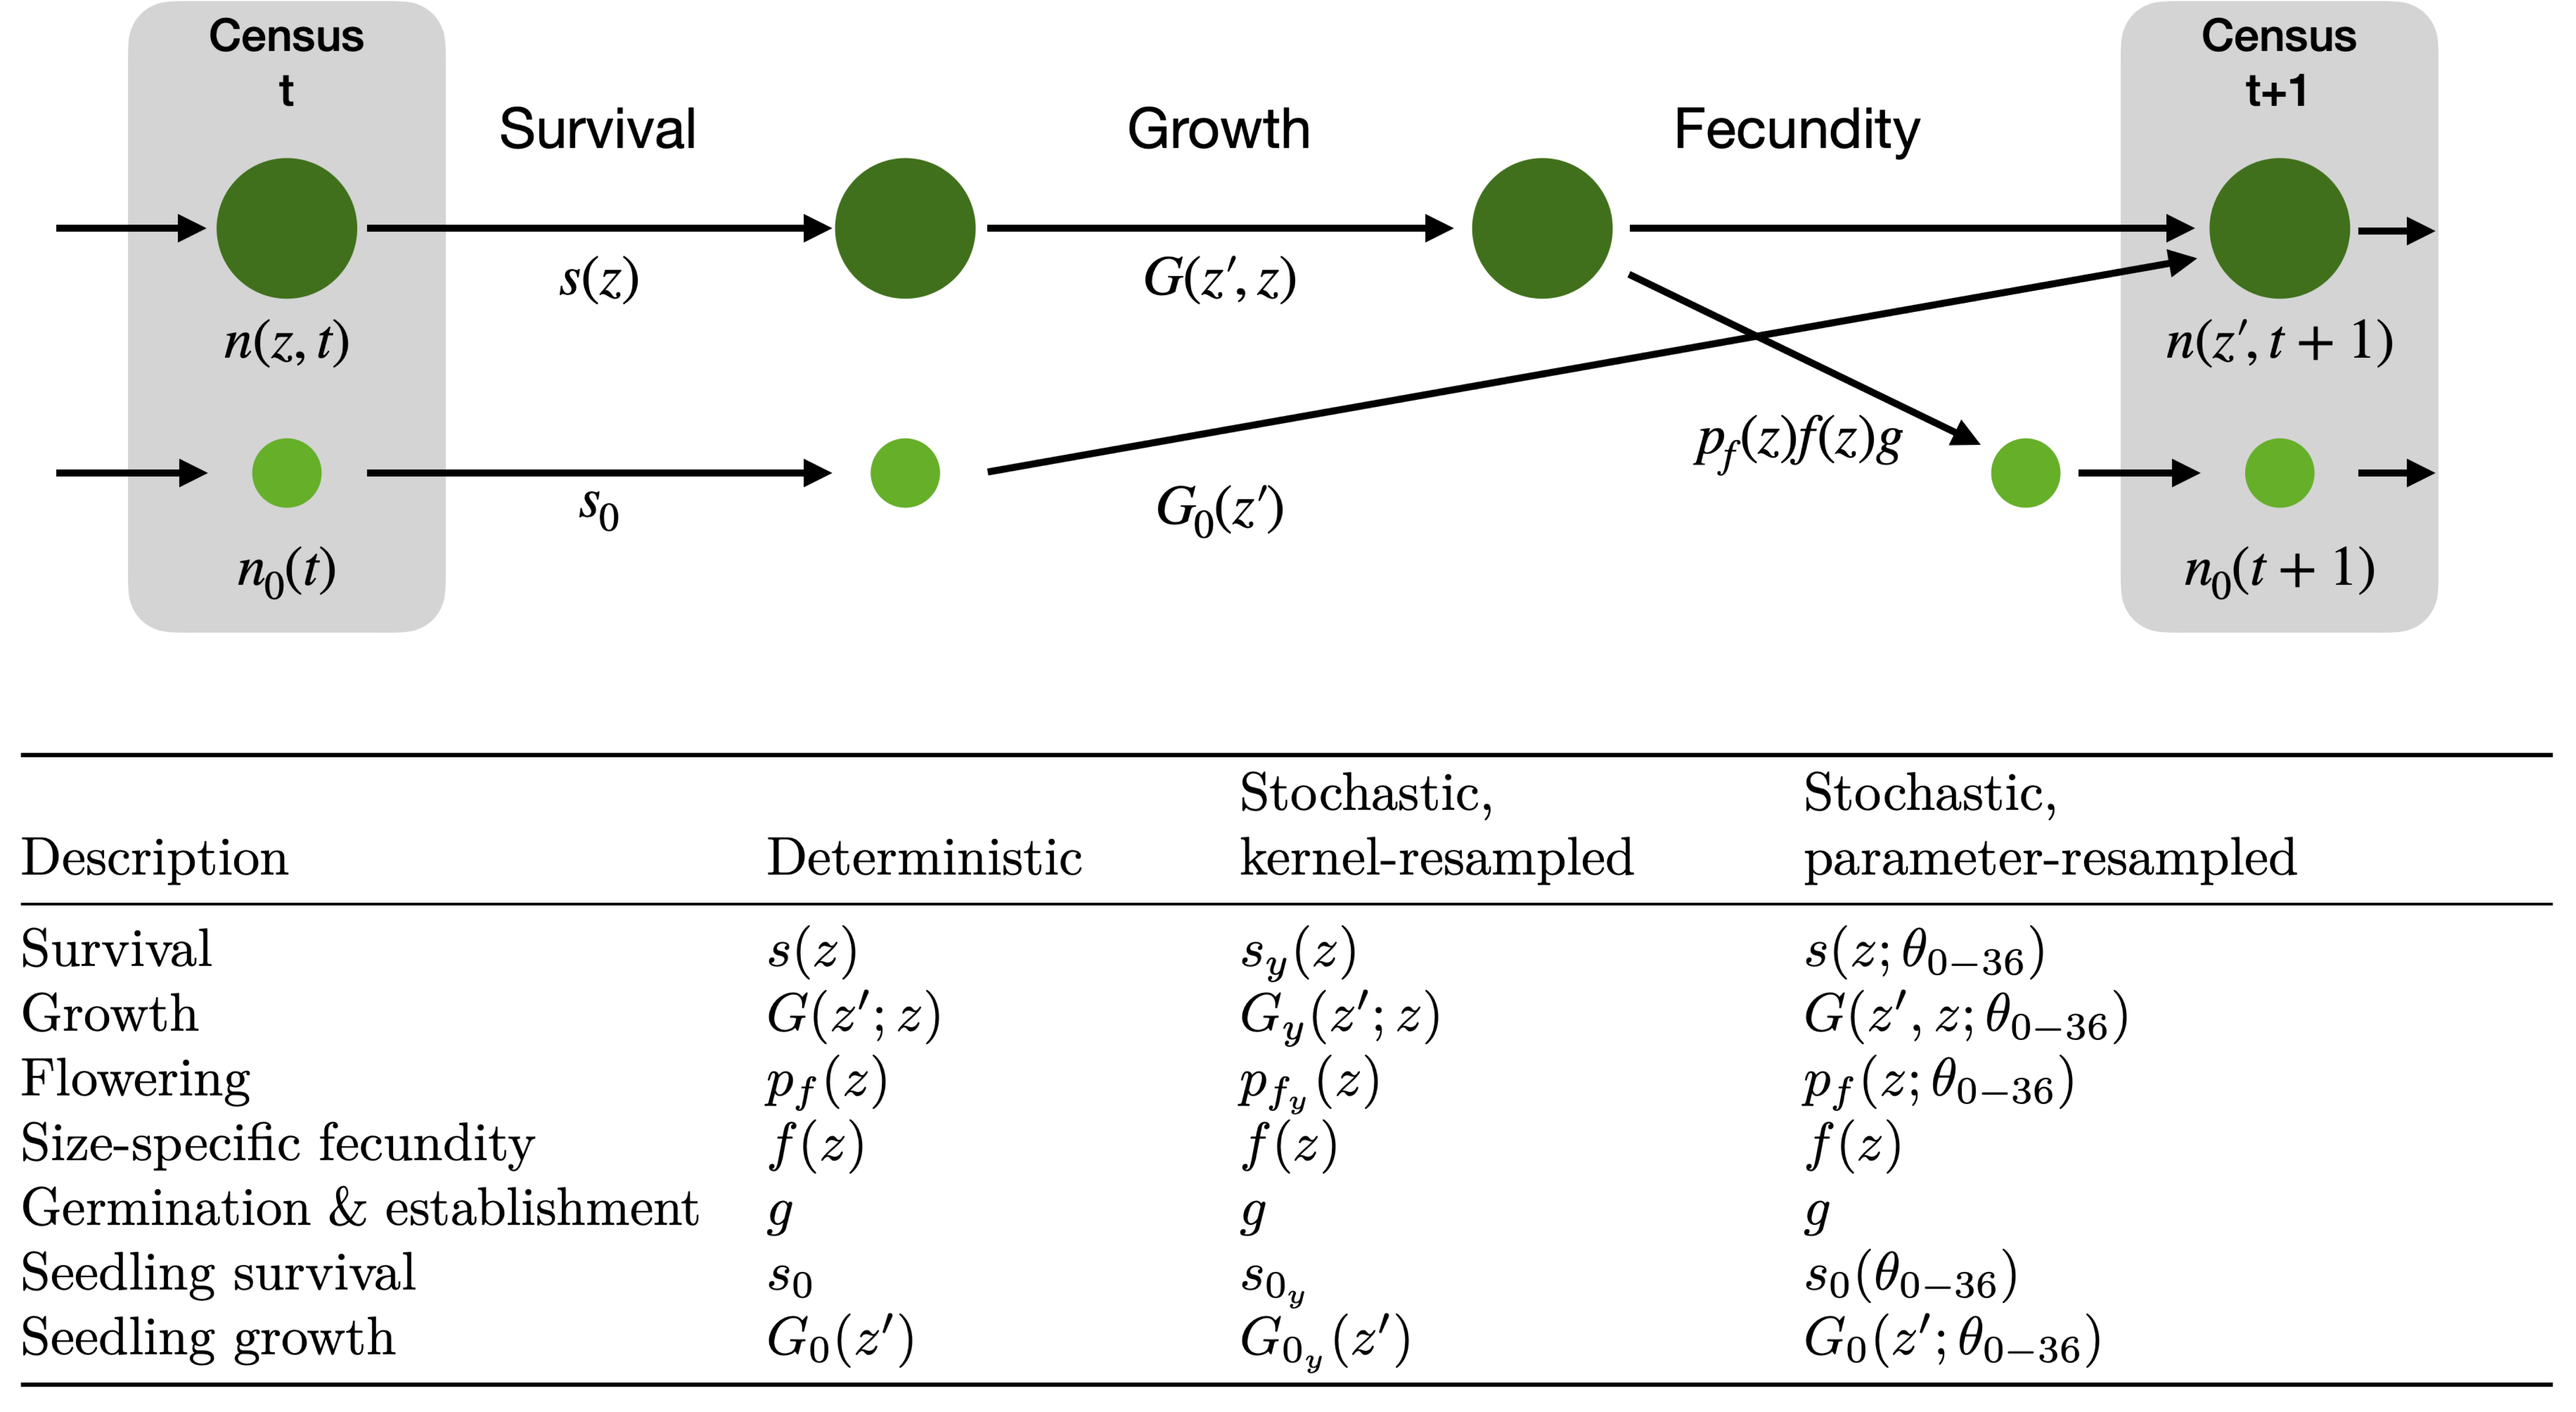
\includegraphics[width=0.85\textwidth,height=\textheight]{/Users/emiliobruna/Dropbox (UFL)/Research/Heliconia/Scott_etal_AmNat/lagged-ipms-ms/docs/figures/lifecycle.png}

}

\caption{\label{fig-lifecycle}Lifecycle diagram of \emph{Heliconia
acuminata}. Each transition is associated with an equation for a vital
rate function. The functions shown on the diagram correspond to those
used to construct a general, density-independent, deterministic IPM. The
table below shows the equivalent equations for stochastic,
kernel-resampled IPMs and stochastic, parameter-resampled IPMs.}

\end{figure}

\newpage

\begin{figure}

{\centering 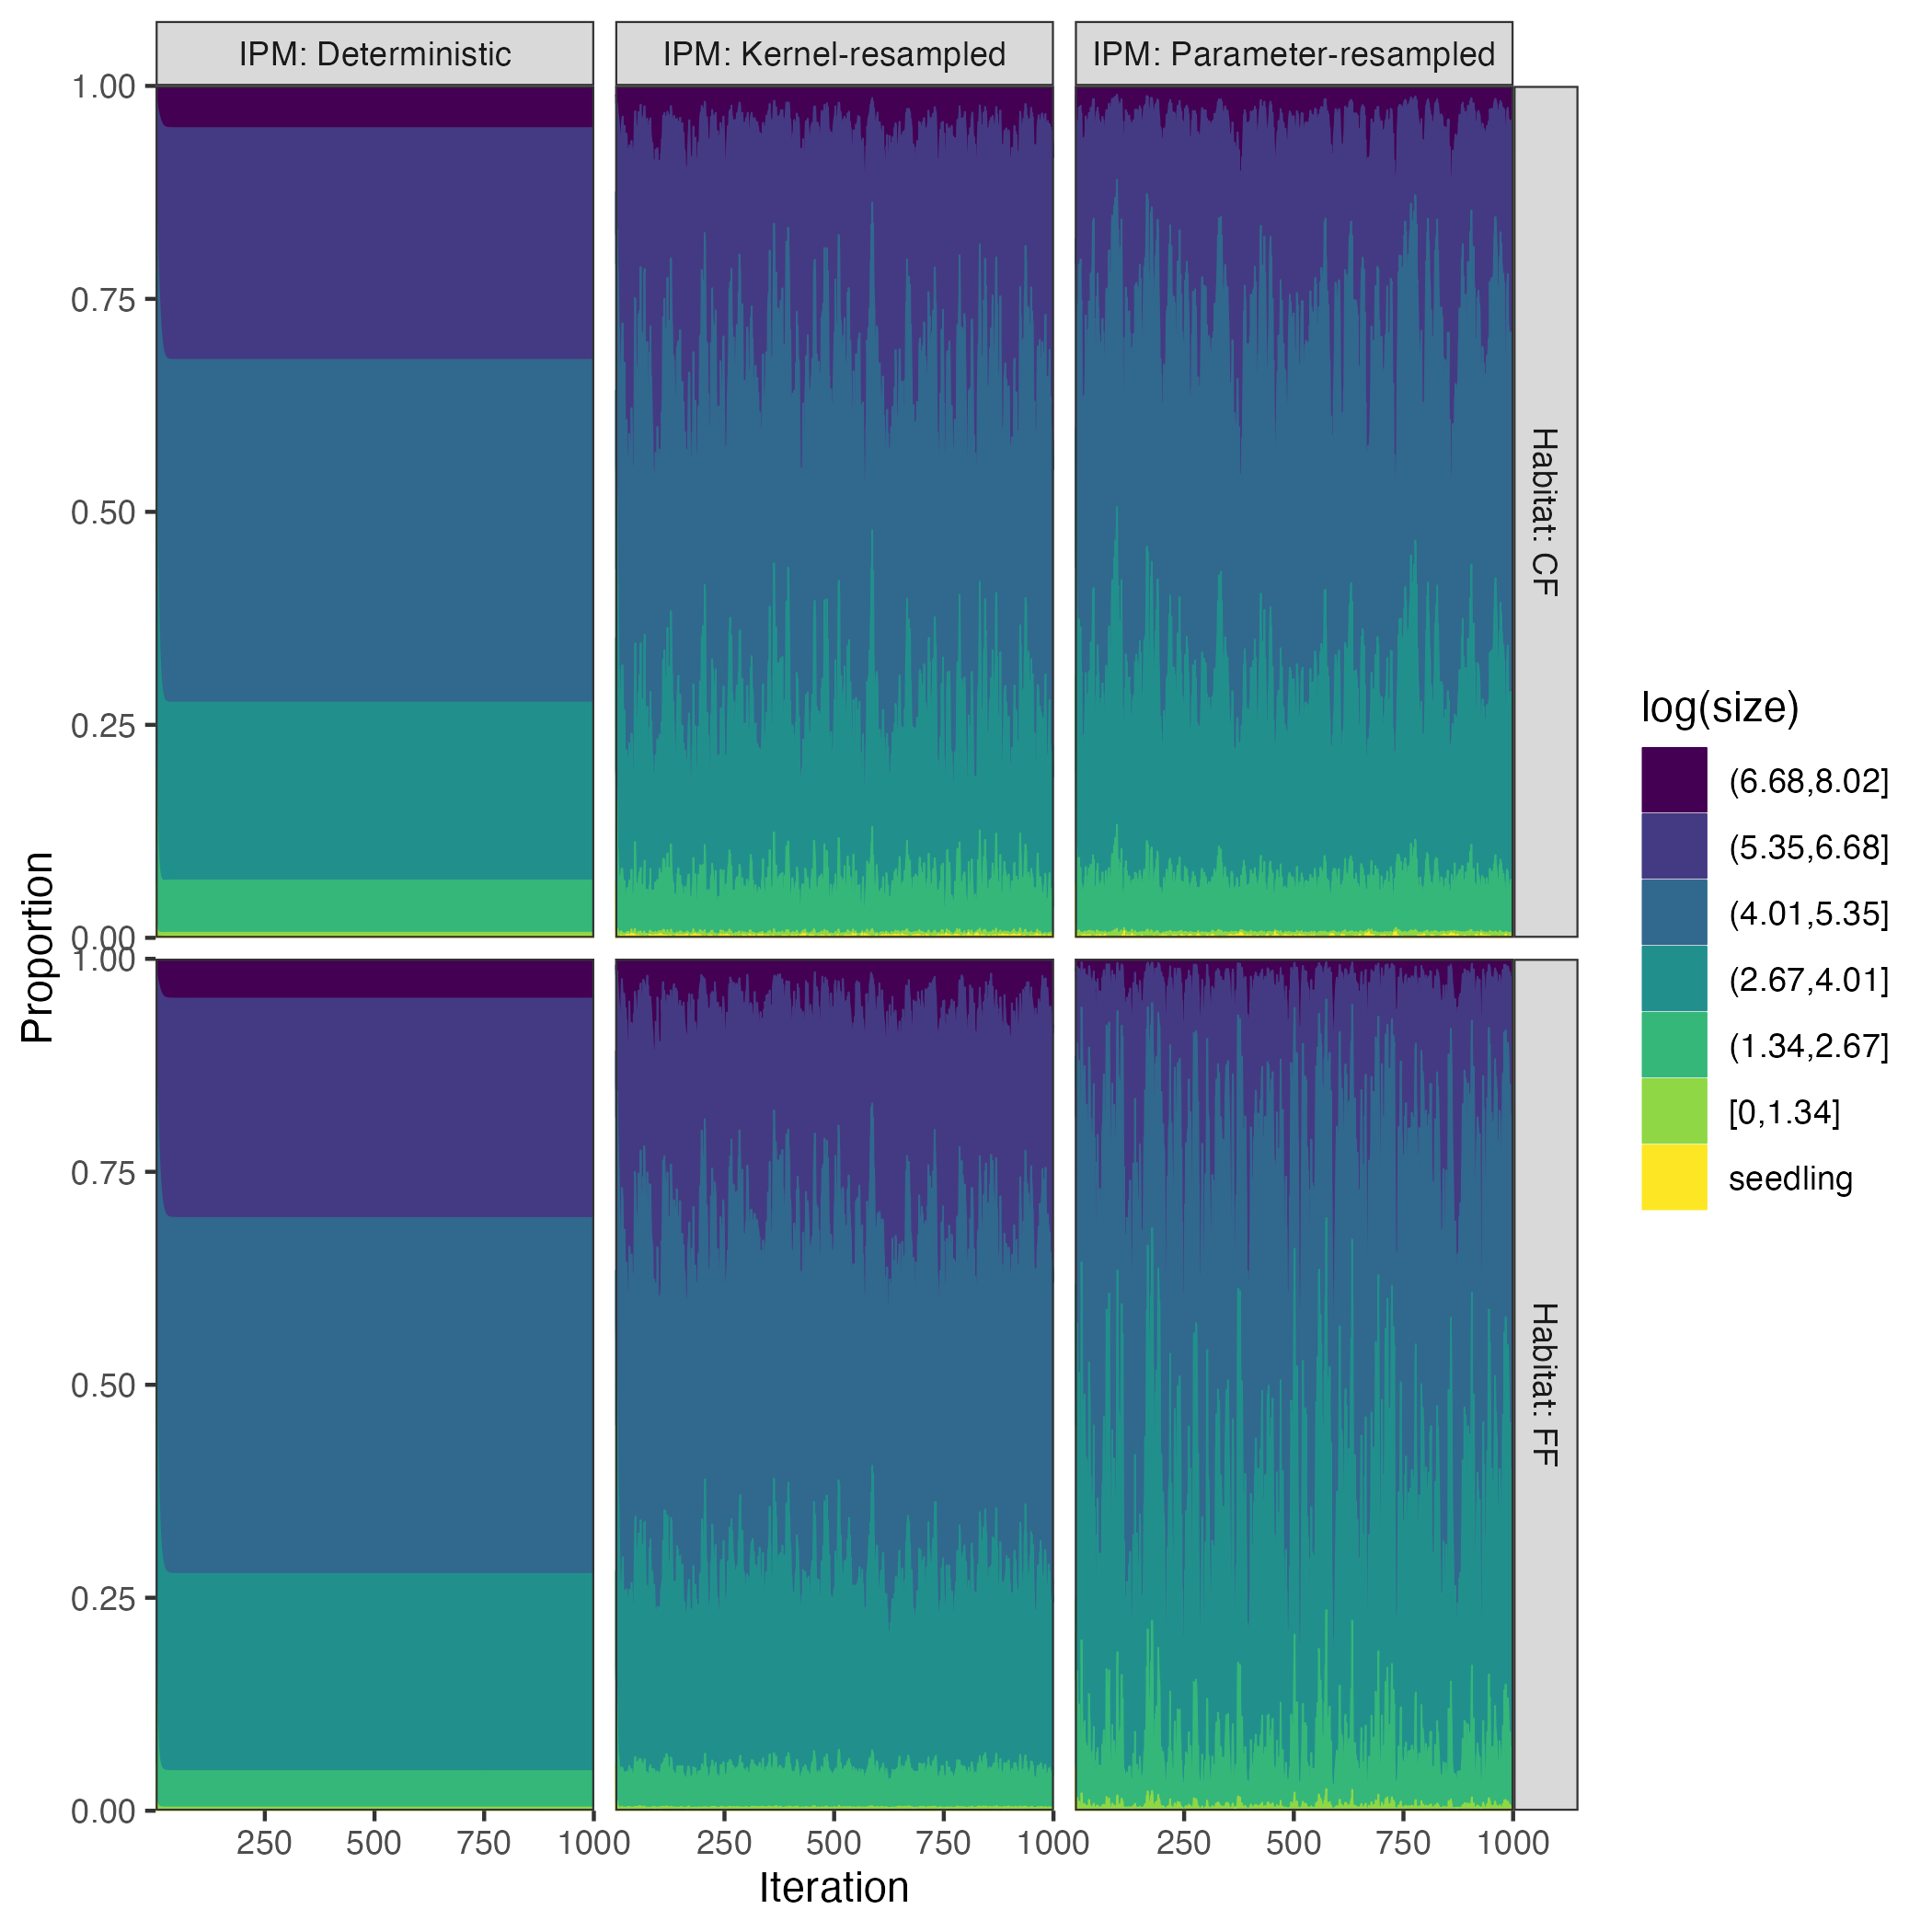
\includegraphics[width=0.85\textwidth,height=\textheight]{/Users/emiliobruna/Dropbox (UFL)/Research/Heliconia/Scott_etal_AmNat/lagged-ipms-ms/docs/figures/pop_states.png}

}

\caption{\label{fig-pop-states}Relative proportions of plant sizes in
the first 250 iterations of the IPM simulations. Stacked area charts (A)
show the relative size/stage distribution of plants in continuous forest
(CF, top row) and forest fragments (FF, bottom row) in each of the three
IPMs (columns). The proportion of each size class in CF and FF for each
iteration is shown in B with the first 30 iterations removed to not
include transient dynamics. A 1:1 line is plotted in black. Size
categories include seedlings (a discrete category in the IPMs),
pre-reproductive 1 (log(size) 0--2.5) that have low average survival
(\textless{} 0.9) and a near 0 probability of flowering,
pre-reproductive 2 (log(size) 2.5--4.5) that have a higher average
survival probabilty (\textgreater{} 0.8) and a near 0 probability of
flowering, reproductive 1 (log(size) 4.5--6) that have a high average
survival probability (\textgreater0.95) and a lower flowering
probability (\textless{} 0.25), and reproductive 2 (log(size) 6+) that
have a high average survival probability (\textgreater0.95) and higher
flowering proability (\textgreater{} 0.2).}

\end{figure}



\end{document}
